% =====================================================================
%  NILES 2026 CAMERA-READY  --  rebuilt from the ACCEPTED paper
%  (EDAS 1571324247) and condensed to 4 pages with the reviewer
%  revisions merged in.
%  Accepted title/abstract/intro (incl. self-citations [3]-[5]),
%  related work, RQ framing and reference list preserved. Both schematic
%  figures are included (U-Net architecture = Fig. 1; distillation
%  framework = Fig. 2) and the reviewer revisions are merged.
%  Toggle: \anonymousfalse = camera-ready (authors), \anonymoustrue = review.
% =====================================================================
\documentclass[conference,a4paper]{IEEEtran}
\IEEEoverridecommandlockouts
\usepackage{cite}
\usepackage{amsmath,amssymb,amsfonts}
\usepackage{graphicx}
\usepackage{subcaption}
\usepackage{textcomp}
\usepackage{xcolor}
\usepackage{booktabs}
\usepackage{tikz}
\usetikzlibrary{positioning, arrows.meta, calc}
\graphicspath{{figures/}}

% tighten float/text separation to fit the 4-page limit
\setlength{\textfloatsep}{4pt plus 1pt minus 1pt}
\setlength{\dbltextfloatsep}{4pt plus 1pt minus 1pt}
\setlength{\floatsep}{4pt plus 1pt minus 1pt}
\setlength{\dblfloatsep}{4pt plus 1pt minus 1pt}

\newif\ifanonymous
\anonymousfalse   % <<< camera-ready (authors shown); \anonymoustrue for anonymous review

\begin{document}

\title{Edge-Efficient WiFi Indoor Localization via\\ Lightweight Deep Learning and Knowledge Distillation}

\ifanonymous
\author{\IEEEauthorblockN{Anonymous submission}\IEEEauthorblockA{Paper submitted to NILES 2026 for double-blind review}}
\else
\author{%
\IEEEauthorblockN{Abdulrahman M. A. Ebrahim, Ahmed E. A. Haggag,\\ Fadwa Y. K. Mahmoud, and Ehab H. Elshazly}
\IEEEauthorblockA{\textit{Egypt-Japan University of Science and Technology (E-JUST)}, Alexandria, Egypt\\
\{abdulrahman.ebrahim, ahmed.emadeldin, fadwa.khalil, ehab.elshazly\}@ejust.edu.eg}
}
\fi

\maketitle

\begin{abstract}
Accurate WiFi indoor localization is increasingly required for edge AI applications such as robots, smart factories, and healthcare monitoring, yet state-of-the-art deep models are too computationally expensive for resource-constrained devices. This paper investigates whether lightweight neural networks combined with knowledge distillation can achieve competitive localization while substantially reducing cost. Using the public WILD dataset, we systematically evaluate four lightweight student architectures (MobileNetV2, MobileNetV2-UNet, TinyCNN, and Mamba) against the Deep Localization (DLoc) teacher in terms of accuracy, robustness to corrupted Channel State Information (CSI), cross-session generalization, statistical stability, and computational efficiency. The best model, a distilled MobileNetV2-UNet, has only 2.41 million parameters, a $6.8\times$ size reduction and $56\times$ fewer FLOPs than DLoc, while matching its published median localization error of 0.64\,m. We further show that knowledge distillation's benefits are capacity-dependent, improving robustness and cross-session generalization rather than in-distribution accuracy, and only above roughly two million parameters. The distilled model achieves the best zero-shot performance on unseen environments, demonstrating that accurate, robust, and efficient WiFi localization does not require large deep neural networks.
\end{abstract}

\begin{IEEEkeywords}
Indoor localization, WiFi, Channel State Information (CSI), Knowledge distillation, CNN, U-Net.
\end{IEEEkeywords}

\section{Introduction}
GPS has long provided reliable positioning outdoors, but its accuracy vanishes inside buildings. Indoor localization has therefore been an active research topic for the last two decades, supporting applications that range from tracking factory assets~\cite{digitaltwin2025framework} to guiding robots and monitoring patients.

The leading approach is WiFi-based localization, which analyzes Channel State Information (CSI) from access points (APs)~\cite{ayyalasomayajula2020deep} to obtain precise estimates of the time-of-flight (ToF) and angle-of-arrival (AoA) of incoming signals---sufficient for sub-meter accuracy. The state of the art, DLoc~\cite{ayyalasomayajula2020deep}, uses a deep learning model to translate this CSI data into a heatmap of the device's location on the floor plan.

Deep learning has achieved strong results in dense prediction and intelligent sensing through effective feature representations and carefully designed optimization objectives, including Gaussian-weighted feature modeling for monocular depth estimation~\cite{elshazly2019gaussian}, appearance-aware optimization for dense prediction~\cite{elshazly2019appearance}, and nonlinear loss integration for novel-view synthesis~\cite{elshazly2024nonlinear}. Building on these architecture- and objective-driven design principles, the present work extends them to CSI-based indoor localization for resource-constrained edge AI systems.

However, DLoc has a significant limitation: it requires a large training dataset and a ResNet model with 16.5 million parameters---too demanding for standard gateways, access points, or smartphones. We investigate whether ``student'' models---smaller, more efficient architectures---can deliver comparable performance without this overhead.

The main contributions are: (i)~lightweight architectures for CSI-based localization suited to edge deployment; (ii)~a study of distillation across student capacities, identifying a threshold below which it no longer helps; (iii)~a comprehensive evaluation of accuracy, robustness, cross-session generalization, stability, and efficiency on WILD; and (iv)~a distilled MobileNetV2-UNet matching DLoc at $6.8\times$ fewer parameters, $56\times$ less computation, and ${\sim}10\times$ lower CPU time.

\section{Related Work}
Indoor localization has been extensively studied using WiFi CSI, which reuses existing infrastructure without dedicated hardware. DLoc~\cite{ayyalasomayajula2020deep} transforms CSI into localization heatmaps with convolutional networks at sub-meter accuracy. Recent work explores transformers for non-line-of-sight settings~\cite{masrur2025transforming}, meta-learning~\cite{owfi2023meta}, few-shot learning~\cite{tiku2023fewshot}, domain adaptation~\cite{jiao2025robust}, adaptive AoA estimation~\cite{adaptiveaoa2026learning}, explainability~\cite{gufran2025towards}, and data augmentation~\cite{serbetci2024wireless}, but generally relies on increasingly complex networks hard to deploy on edge devices.

Research has therefore turned to lightweight deep learning and edge AI. Efficient architectures such as MobileNetV2~\cite{sandler2018mobilenetv2}, residual learning~\cite{he2016resnet}, and encoder--decoder networks with skip connections~\cite{ronneberger2015unet} offer strong accuracy--complexity trade-offs, while state-space models such as Mamba~\cite{gu2023mamba,visualmamba2024survey} are efficient alternatives to transformers; lightweight inference is likewise central to green wireless sensing~\cite{greenwireless2026survey} and TinyML-enabled IoT~\cite{tinyml2022iot}.

Knowledge distillation compresses networks by transferring knowledge from a high-capacity teacher to a lightweight student~\cite{hinton2015distilling}, and has been applied to dense prediction such as object detection~\cite{zheng2023localization} and cross-modal localization~\cite{nazaraliyev2025mambaloc}. However, the interaction between student capacity, distillation, robustness to corrupted CSI, and cross-session generalization for WiFi localization remains largely unexplored. Unlike prior work, we jointly study lightweight architectures and distillation, providing practical design guidelines for edge deployment.

\section{Methodology}
\subsection{Overview of the DLoc Framework}
DLoc~\cite{ayyalasomayajula2020deep} formulates localization as heatmap prediction: four AoA--ToF images, one per access point, are processed by a ResNet encoder and two decoders---a location decoder and a consistency (offset) decoder---totaling approximately 16.5\,M parameters.

\subsection{WILD Dataset}
The WILD dataset (Jacobs Hall, UCSD) has five sessions: two July sessions give 17{,}574 training and 4{,}260 in-distribution test samples; three August sessions add harder changes (rearranged furniture, 11{,}201; different furniture, 8{,}754; aluminum reflector, 5{,}486). For the leave-one-session-out (LOSO) protocol~\cite{ayyalasomayajula2020deep}, three folds each train on the two July plus two August sessions and test on the held-out August session.

\subsection{Student Network Architectures}
All students share the teacher's input and output; Table~\ref{tab:models} lists the high-performing ones and their cost. MobileNetV2 (2.27\,M) uses depthwise separable convolutions; MobileNetV2-UNet (2.41\,M) adds U-Net skip connections concatenating encoder and decoder feature maps (Fig.~\ref{fig:unet}). Two highly compact models---Mamba (0.65\,M, 1D state-space) and TinyCNN (47\,K, $351\times$ compression)---probe the low-capacity end; their results appear in the lower sub-block of Table~\ref{tab:indist}.

\begin{table}[t]
\caption{High-Performing Models and Their Computational Cost (Batch Size 1; DLoc = Test-Time Path: Encoder + Location Decoder).}
\label{tab:models}
\centering
\scriptsize
\setlength{\tabcolsep}{4pt}
\resizebox{\columnwidth}{!}{%
\begin{tabular}{@{}lrcrrr@{}}
\toprule
\textbf{Model} & \textbf{Params} & \textbf{Compr.} & \textbf{FLOPs} & \textbf{CPU (ms)} & \textbf{GPU (ms)} \\
\midrule
DLoc (teacher)   & 16.5M  & $1\times$   & 81.06G & 270.9 & 16.2 \\
MobileNetV2      & 2.27M  & $7.2\times$ & 1.28G  & 17.9  & 6.3 \\
MobileNetV2-UNet & 2.41M  & $6.8\times$ & 1.45G  & 27.2  & 4.5 \\
\bottomrule
\end{tabular}}
\end{table}

% Fig. 1: single-column, folded into two rows (U-shape) so it is larger and more
% legible while fitting one column and using the free vertical space on page 4.
\begin{figure}[t]
\centering
\resizebox{\columnwidth}{!}{% ============================================================================
%  MobileNetV2-UNet architecture — \input-able body (no \documentclass).
%  Requires in the master preamble: \usepackage{tikz} and
%  \usetikzlibrary{positioning, arrows.meta, calc}.  Colours are defined here
%  so the figure is self-contained.  Layer specs from code/models/student_unet.py.
% ============================================================================
\definecolor{cEnc}{RGB}{142,202,230}
\definecolor{cBottle}{RGB}{33,102,172}
\definecolor{cDec}{RGB}{69,123,157}
\definecolor{cHead}{RGB}{188,108,37}
\definecolor{cSkip}{RGB}{42,157,143}
\definecolor{cIO}{RGB}{230,57,70}

% Two-row (U-shape) layout: encoder flows left->right along the top, the
% bottleneck turns down at the right, and the decoder flows right->left along the
% bottom.  Skip connections run vertically between vertically-aligned levels.
\begin{tikzpicture}[
  font=\small,
  >={Stealth[length=2.4mm]},
  block/.style={rectangle, rounded corners=2pt, draw=black!70, thick,
                minimum height=12mm, minimum width=15mm, align=center,
                text=white, font=\normalsize\bfseries},
  enc/.style={block, fill=cEnc, text=black},
  bottle/.style={block, fill=cBottle},
  dec/.style={block, fill=cDec},
  head/.style={block, fill=cHead},
  io/.style={rectangle, rounded corners=1pt, draw=black!70, thick,
             minimum height=14mm, minimum width=15mm, align=center,
             fill=cIO!12, font=\normalsize},
  flow/.style={->, black!75, thick},
  skipline/.style={->, cSkip, very thick, dashed},
]
% ---- Encoder row (top, left -> right) ----
\node[io] (in) {Input\\$4{\times}161{\times}361$};
\node[enc,    right=6mm of in]  (inc) {inc\\$4{\to}32$\\/2};
\node[enc,    right=6mm of inc] (e1)  {enc1\\$24$};
\node[enc,    right=6mm of e1]  (e2)  {enc2\\$32$};
\node[enc,    right=6mm of e2]  (e3)  {enc3\\$96$};
\node[bottle, right=6mm of e3]  (e4)  {enc4\\$320$};
% ---- Decoder row (bottom) aligned under the encoder for vertical skips ----
\node[dec,  below=16mm of e3] (d1) {dec1\\$416{\to}128$};
\node[dec,  below=16mm of e2] (d2) {dec2\\$160{\to}64$};
\node[dec,  below=16mm of e1] (d3) {dec3\\$88{\to}32$};
\node[head, below=16mm of inc](hd) {head\\$32{\to}1$\\Sigmoid};
\node[io,   below=16mm of in] (out){Output\\$1{\times}161{\times}361$};
% ---- Encoder flow ----
\draw[flow] (in)--(inc); \draw[flow] (inc)--(e1); \draw[flow] (e1)--(e2);
\draw[flow] (e2)--(e3);  \draw[flow] (e3)--(e4);
% ---- Bottleneck turns down to the decoder ----
\draw[flow] (e4.south) to[out=-90,in=0] (d1.east);
% ---- Decoder flow (right -> left) ----
\draw[flow] (d1)--(d2); \draw[flow] (d2)--(d3); \draw[flow] (d3)--(hd); \draw[flow] (hd)--(out);
% ---- Skip connections (vertical, dashed) ----
\draw[skipline] (e3.south) -- node[right=1pt,font=\small,text=cSkip]{skip 96} (d1.north);
\draw[skipline] (e2.south) -- node[right=1pt,font=\small,text=cSkip]{skip 32} (d2.north);
\draw[skipline] (e1.south) -- node[right=1pt,font=\small,text=cSkip]{skip 24} (d3.north);
\node[text=black!60, font=\small, above=1.5mm of e2.north]
      {MobileNetV2 encoder (pretrained, 4-ch input)};
\node[text=black!60, font=\small, below=1.5mm of d3.south]
      {U-Net decoder (upsample $+$ skip concat)};
\end{tikzpicture}
}
\caption{The MobileNetV2-UNet student: a MobileNetV2 encoder (top) and U-Net decoder (bottom) linked by skip connections.}
\label{fig:unet}
\end{figure}

\begin{figure}[t]
\centering
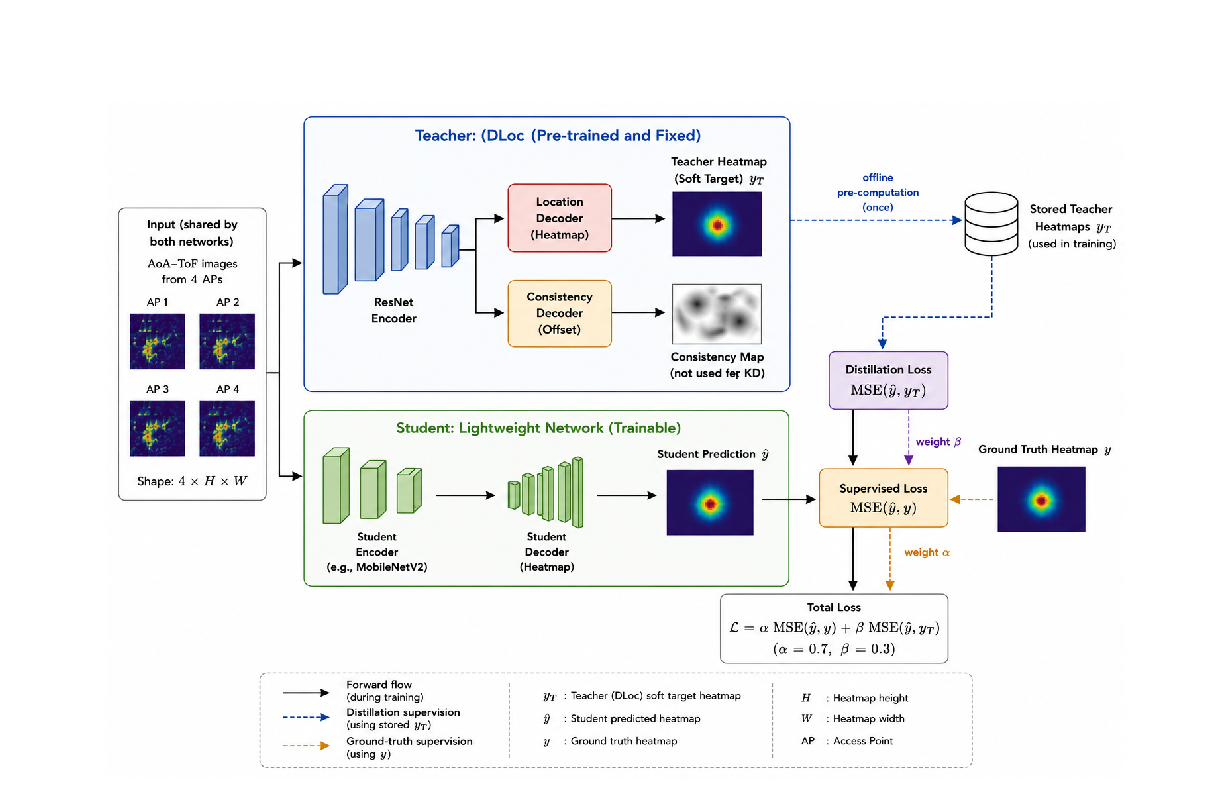
\includegraphics[width=\columnwidth]{fig2_framework.pdf}
\caption{Edge-efficient distillation framework: the fixed DLoc teacher's soft heatmap, pre-computed offline, supervises the lightweight student alongside the ground truth; only the student is deployed at inference.}
\label{fig:framework}
\end{figure}

\subsection{Knowledge-Distillation Framework}
As illustrated in Fig.~\ref{fig:framework}, the framework follows a teacher--student paradigm. Unlike classification distillation, which softens class logits with a temperature parameter~\cite{hinton2015distilling}, the DLoc teacher already emits a spatial \emph{soft target}: a single-channel heatmap $y_T$ whose probability mass is spread around the estimated location, encoding the teacher's spatial uncertainty and its implicit weighting of the four APs---information absent from the one-hot label $y$. Each student is trained in two modes: \emph{standalone}, supervised only by the ground truth ($\mathrm{MSE}(\hat{y},y)$); and \emph{distilled}, minimizing a weighted sum of that loss and a distillation loss matching the teacher heatmap:
\begin{equation}
\mathcal{L} = \alpha\,\mathrm{MSE}(\hat{y}, y) + \beta\,\mathrm{MSE}(\hat{y}, y_T),
\label{eq:loss}
\end{equation}
where both terms are pixel-wise MSE over the output heatmap and $(\alpha,\beta){=}(0.7,0.3)$ keep the ground-truth term dominant while using the teacher as a regularizer ($\beta{=}0$ recovers the standalone objective). The teacher heatmaps $y_T$ are pre-computed offline and cached, so the 16.5\,M-parameter teacher never runs during student training; only the student is deployed at inference.

\subsection{Evaluation Metrics}
The localization error ($e$) is the Euclidean distance between the two heatmap peaks:
\begin{equation}
e = 0.1 \cdot \lVert \arg\max(\hat{y}) - \arg\max(y) \rVert_2 \;\; [\mathrm{m}],
\label{eq:err}
\end{equation}
where the factor of 0.1 converts pixels to meters. Following~\cite{ayyalasomayajula2020deep}, we report the median of $e$ with the 90th (P90) and 99th (P99) percentiles. Because the error is quantized to multiples of $0.1\sqrt{n}$, models can share a median yet differ in distribution, so percentiles better characterize the error.

\section{Implementation}
All models use PyTorch. TinyCNN and MobileNetV2 use Adam (learning rate $10^{-4}$, batch size~64) for 50 epochs; MobileNetV2-UNet trains 120 epochs with cosine-annealing and step-decay; DLoc uses Adam ($\beta_1{=}0.5$) with StepLR ($\gamma{=}0.9$). The best model per architecture is chosen by lowest test error. Training uses rented H100 GPUs; latencies in Table~\ref{tab:models} use a desktop RTX~3060. Because the teacher is not retrained per fold, MobileNetV2-UNet runs standalone under LOSO for comparability with DLoc. All code, weights, logs, and teacher outputs are archived publicly.

\section{Results and Discussion}
We evaluate in-distribution accuracy, robustness to corrupted CSI, cross-session generalization, statistical stability, and the accuracy--efficiency trade-off.

\subsection{In-Distribution Accuracy}
\label{sec:indist}
Table~\ref{tab:indist} reports errors on the held-out Session-2 split; Fig.~\ref{fig:cdf} plots the CDFs. MobileNetV2 achieves the same result as our DLoc reproduction (median 0.707\,m), yet uses $7.2\times$ fewer parameters, evidence that DLoc is over-parameterized in-distribution. TinyCNN (lower sub-block of Table~\ref{tab:indist}) remains far from competitive (3.92\,m standalone, 3.71\,m distilled), indicating a capacity floor of approximately 2 million parameters. MobileNetV2-UNet achieves the lowest median error of 0.640\,m---9.5\% below MobileNetV2 and our DLoc reproduction, and level with DLoc's published 0.64\,m~\cite{ayyalasomayajula2020deep}. Standalone and distilled models share the same median: in-distribution the teacher's outputs match the ground truth, so distillation offers no benefit; this changes out of distribution (Secs.~\ref{sec:robust} and~\ref{sec:cross}). Finally, Mamba was not competitive (median 10.56\,m): its training and test errors rise together from the first epoch---not overfitting but an architectural mismatch, since flattening the 2D heatmaps into 1D sequences destroys spatial locality.

\begin{table}[t]
\caption{In-Distribution Accuracy (Session-2 Test Set, $N{=}4{,}260$; Best in \textbf{Bold}; Published DLoc from~\cite{ayyalasomayajula2020deep}). The Under-Capacity Models (TinyCNN, Mamba) are Reported in the Lower Sub-Block.}
\label{tab:indist}
\centering
\scriptsize
\setlength{\tabcolsep}{4pt}
\resizebox{\columnwidth}{!}{%
\begin{tabular}{@{}lrlccc@{}}
\toprule
\textbf{Model} & \textbf{Params} & \textbf{Mode} & \textbf{Med.\ (m)} & \textbf{P90 (m)} & \textbf{P99 (m)} \\
\midrule
DLoc (published) & 16.5M & ---        & \textbf{0.64} & 1.6 & 3.2 \\
DLoc (our repro) & 16.5M & ---        & 0.707 & ${\sim}1.6$ & ${\sim}4.0$ \\
\midrule
MobileNetV2      & 2.27M & Standalone & 0.707 & 1.616 & 3.992 \\
MobileNetV2      & 2.27M & Distilled  & 0.707 & 1.612 & 4.003 \\
\midrule
MobileNetV2-UNet & 2.41M & St.\ (Cos) & \textbf{0.640} & 1.523 & 2.750 \\
MobileNetV2-UNet & 2.41M & St.\ (Step)& \textbf{0.640} & 1.552 & 2.918 \\
MobileNetV2-UNet & 2.41M & Dist.\ (Cos)& \textbf{0.640} & \textbf{1.513} & \textbf{2.587} \\
\midrule
\multicolumn{6}{@{}l}{\scriptsize\itshape Under-capacity / architecture-mismatch (non-competitive):}\\
Mamba            & 0.65M & Standalone  & 10.56 & 20.0  & 28.3 \\
TinyCNN          & 47K   & Standalone  & 3.922 & 13.919 & 23.244 \\
TinyCNN          & 47K   & Distilled   & 3.706 & 14.784 & 25.101 \\
\bottomrule
\end{tabular}}
\end{table}

\begin{figure}[t]
\centering
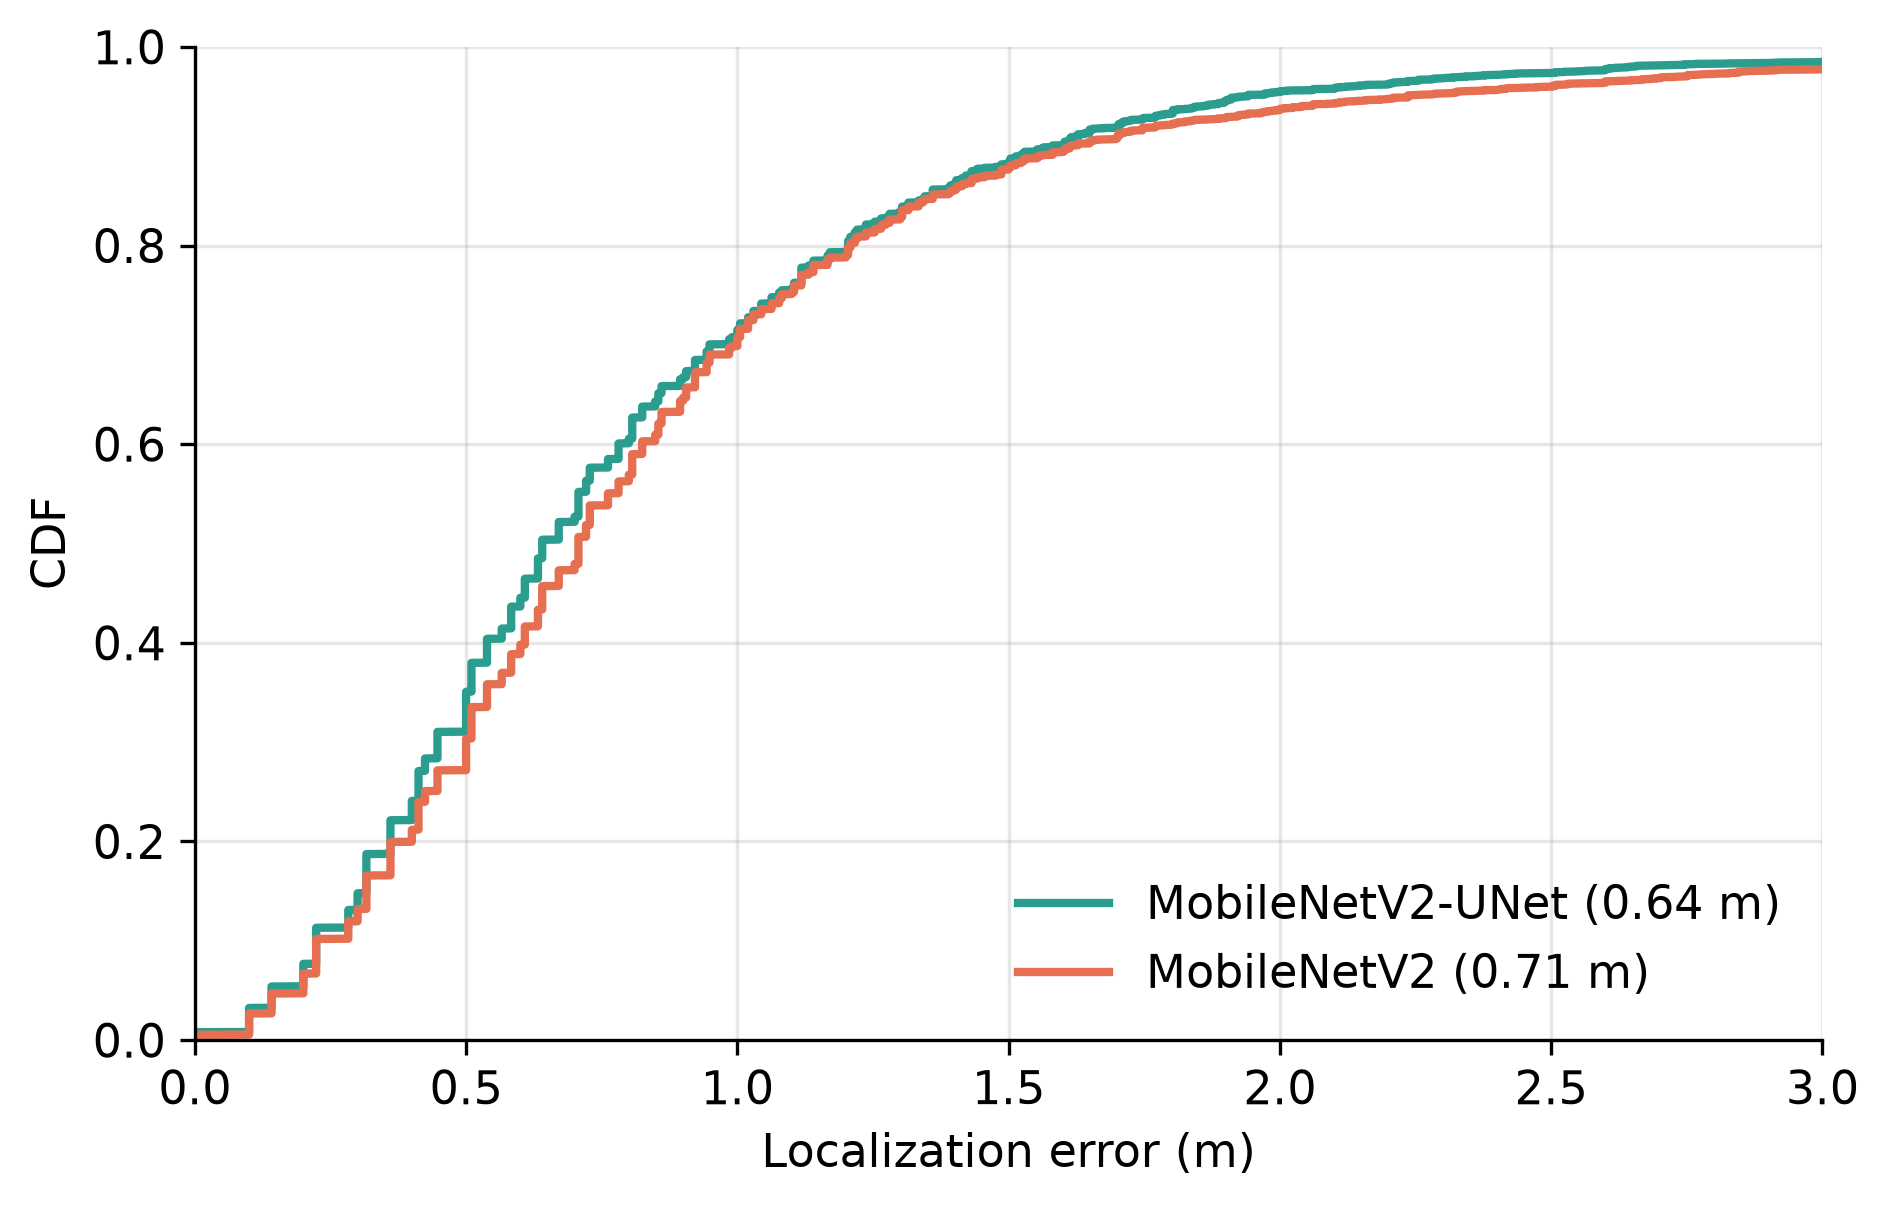
\includegraphics[width=0.5\linewidth]{cdf_fig10b.png}
\caption{CDF of in-distribution localization error for the high-performing models.}
\label{fig:cdf}
\end{figure}

\subsection{Robustness to Corrupted Inputs}
\label{sec:robust}
We corrupt the CSI only at test time: per-AP and random AP dropout, additive Gaussian noise ($\sigma \in \{0.1, 0.2\}$), attenuation, and spatial blur. Table~\ref{tab:robust} shows the Gaussian-noise case. Distillation protects high-capacity students: the standalone MobileNetV2 degrades to 16.4\,m at $\sigma = 0.1$, yet its distilled version degrades only to 4.8\,m ($3.4\times$ better). Skip connections provide a second, independent layer of protection: the standalone MobileNetV2-UNet reaches 3.0\,m ($5.5\times$ better than the standalone MobileNetV2). The two mechanisms are complementary rather than additive: the distilled MobileNetV2-UNet gains no extra Gaussian-noise robustness from distillation (3.000\,m vs.\ 3.469\,m), but distillation does improve its robustness to AP dropout. Distillation also has a capacity threshold: on the 47\,K TinyCNN it leaves noise robustness unchanged (9.46 vs.\ 9.44\,m) yet worsens AP-dropout robustness (random 1-AP: 7.9 to 13.6\,m), as the small model spends its capacity imitating the teacher's AP fusion rather than resisting dropout.

\begin{table}[t]
\caption{Gaussian-Noise Robustness of the High-Performing Models ($\sigma = 0.1$).}
\label{tab:robust}
\centering
\scriptsize
\setlength{\tabcolsep}{6pt}
\begin{tabular}{@{}llcc@{}}
\toprule
\textbf{Model} & \textbf{Mode} & \textbf{Median (m)} & \textbf{P90 (m)} \\
\midrule
MobileNetV2      & Standalone & 16.368 & 20.939 \\
MobileNetV2      & Distilled  & 4.769  & 12.310 \\
MobileNetV2-UNet & Standalone & \textbf{3.000} & \textbf{8.310} \\
MobileNetV2-UNet & Distilled  & 3.469  & 10.473 \\
\bottomrule
\end{tabular}
\end{table}

\subsection{Cross-Session Generalization}
\label{sec:cross}
The LOSO results over three random seeds (Table~\ref{tab:loso}) show that the 2.41\,M-parameter MobileNetV2-UNet is competitive with the 16.5\,M-parameter DLoc: it matches DLoc on the different-furniture fold (0.822\,m vs.\ 0.82\,m), is within 0.14\,m of DLoc on the remaining folds, has essentially the same mean P90 (2.374\,m vs.\ 2.33\,m), and has a lower P90 on the challenging reflector fold (2.489\,m vs.\ 2.77\,m). The residual gap on the reflector fold is expected: DLoc's offset decoder regularizes estimates across APs---beneficial under specular reflection---whereas the single-decoder student has none. The LOSO students run standalone because the teacher is not retrained per fold, so no in-domain distillation targets exist for held-out sessions. A \emph{fold-specific} teacher (DLoc retrained per fold) would supply such targets; since distillation already helps the zero-shot U-Net on the shifted reflector session (Table~\ref{tab:zeroshot}), it would be expected to \emph{further} lower the LOSO error, not raise it. The standalone results are thus a conservative bound; we avoid a per-fold 16.5\,M teacher as it would defeat the study's compression objective.

We also train the models on only the two July sessions and evaluate zero-shot on the never-seen August sessions (Table~\ref{tab:zeroshot}). The distilled U-Net has the lowest median and P90 on each August session; on the most difficult (reflector) session its median is 1.281\,m, versus 1.334\,m for the standalone model and 1.442\,m for the best MobileNetV2. Thus, the distilled MobileNetV2-UNet is recommended as the deployment configuration.

\begin{table}[t]
\caption{Leave-One-Session-Out vs.\ Published DLoc (Mean$\pm$Std, 3 Seeds; Ours = Standalone MobileNetV2-UNet).}
\label{tab:loso}
\centering
\scriptsize
\setlength{\tabcolsep}{3pt}
\resizebox{\columnwidth}{!}{%
\begin{tabular}{@{}lcccc@{}}
\toprule
\textbf{Held-out session} & \textbf{Med.\ (ours)} & \textbf{Med.\ (paper)} & \textbf{P90 (ours)} & \textbf{P90 (paper)} \\
\midrule
Aug16\_1 (furn.)        & $0.852\pm0.044$ & 0.71 & $1.839\pm0.067$ & 1.71 \\
Aug16\_3 (diff.\ furn.) & $0.822\pm0.040$ & 0.82 & $2.793\pm0.140$ & 2.52 \\
Aug16\_4\_ref (refl.)   & $1.116\pm0.016$ & 1.05 & $2.489\pm0.030$ & 2.77 \\
\midrule
Mean                    & 0.930 & 0.86 & 2.374 & 2.33 \\
\bottomrule
\end{tabular}}
\end{table}

\begin{table}[t]
\caption{Zero-Shot Cross-Session Accuracy (July-Only Training). Cells: Median\,/\,P90 (m); Best in \textbf{Bold}.}
\label{tab:zeroshot}
\centering
\scriptsize
\setlength{\tabcolsep}{3pt}
\resizebox{\columnwidth}{!}{%
\begin{tabular}{@{}llccc@{}}
\toprule
\textbf{Model} & \textbf{Mode} & \textbf{Aug16\_1} & \textbf{Aug16\_3} & \textbf{Aug16\_4\_ref} \\
\midrule
MobileNetV2      & Standalone & 1.118\,/\,3.138 & 1.204\,/\,3.471 & 1.500\,/\,3.367 \\
MobileNetV2      & Distilled  & 1.118\,/\,3.228 & 1.204\,/\,3.342 & 1.442\,/\,3.711 \\
MobileNetV2-UNet & Standalone & 1.063\,/\,2.508 & 1.005\,/\,3.704 & 1.334\,/\,3.301 \\
MobileNetV2-UNet & Distilled  & \textbf{1.020\,/\,2.319} & \textbf{1.005\,/\,2.608} & \textbf{1.281\,/\,3.002} \\
\bottomrule
\end{tabular}}
\end{table}

\subsection{Statistical Stability and Efficiency}
To confirm the gains are not seed noise, DLoc was trained with three seeds for 120 epochs. Its median of $0.875 \pm 0.036$\,m---a coefficient of variation (CoV) of 4.1\%---exceeds the 50-epoch value because the StepLR schedule ($\gamma{=}0.9$) never decays the learning rate to zero over 120 epochs. Still, the MobileNetV2-UNet's 0.640\,m median is 6.5 standard deviations below this mean; the P99 varies far more across seeds (CoV 52\%). In efficiency (Table~\ref{tab:models}), the MobileNetV2-UNet uses $56\times$ fewer GFLOPs than DLoc (1.45 vs.\ 81.06), is $10\times$ faster on CPU (27.2 vs.\ 270.9\,ms), and $3.6\times$ faster on GPU---so its accuracy gains come at no computational cost, a strong fit for edge deployment.

\section{Conclusion}
We investigated whether high WiFi localization accuracy requires large networks. DLoc can be compressed by nearly an order of magnitude while matching its accuracy: MobileNetV2 (2.27\,M) matches our reproduced DLoc (0.707\,m), and MobileNetV2-UNet (2.41\,M) reaches the published 0.640\,m median at $6.8\times$ fewer parameters, $56\times$ fewer FLOPs, and ${\sim}10\times$ lower CPU time. Two insights emerge: distillation is capacity-dependent, aiding robustness and cross-session generalization---not in-distribution accuracy---only above ${\sim}2$\,M parameters; and architecture matters, as skip connections resist noisy CSI while distillation helps most under AP dropout. The distilled MobileNetV2-UNet best balances accuracy, robustness, generalization, and efficiency, and is our recommended edge configuration. Future work will validate on edge devices, collect a CSI dataset
\ifanonymous
in a different building
\else
on the E-JUST campus
\fi
to evaluate cross-building generalization, investigate corruption-aware training, and extend the multi-seed analysis to all student architectures.

% uniform reference-list spacing (equal gap between every line) within the 4-page limit
\let\oldthebibliography\thebibliography
\renewcommand{\thebibliography}[1]{\oldthebibliography{#1}\scriptsize\raggedright\setlength{\itemsep}{0pt}\setlength{\parsep}{0pt}}
\bibliographystyle{IEEEtran}
\bibliography{references}

\end{document}
